\documentclass{article}
\usepackage{tikz}
\usetikzlibrary{positioning}
\usetikzlibrary{calc}
\usetikzlibrary{arrows,shapes,backgrounds}
\begin{document}
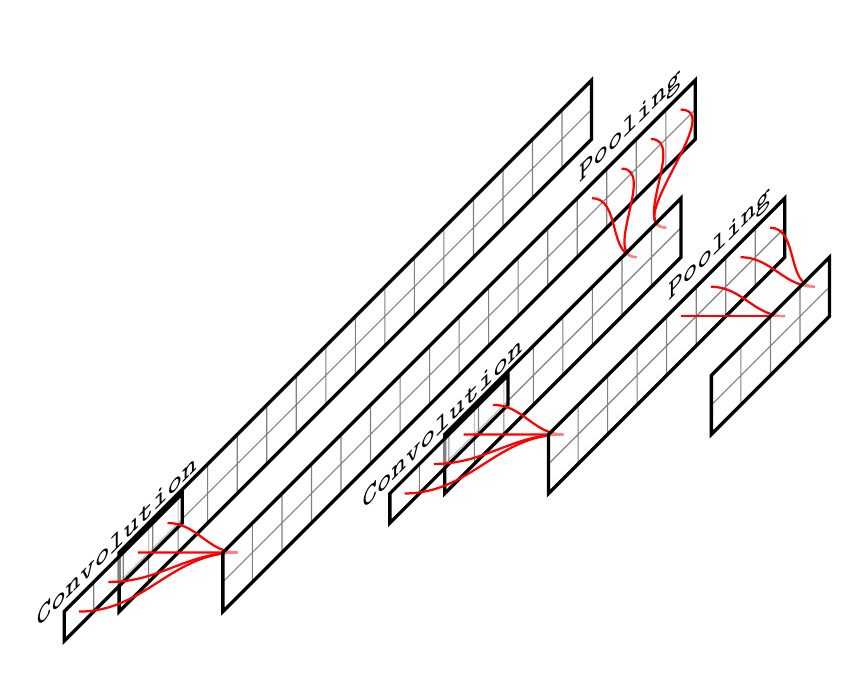
\begin{tikzpicture}[scale=1.5,every node/.style={minimum size=1cm},on grid]
    \begin{scope}[
            yshift=0, xshift=-100, every node/.append style={
            yslant=1,xslant=0},yslant=1,xslant=0]
        \fill[white,fill opacity=0.9] (0,0) rectangle (4,0.5);
        \draw[step=2.5mm, thin, gray] (0,0) grid (4,0.5); %defining grids
        \draw[black,very thick] (0,0) rectangle (4,0.5);%marking borders      
		\pgfkeys{/pgf/number format/.cd, fixed, zerofill, precision =1} 
    \end{scope}
    
    \begin{scope}[
            yshift=0.25cm, xshift=-99, every node/.append style={
            yslant=1,xslant=0},yslant=1,xslant=0]
        \fill[white,fill opacity=0.5] (-0.5,0) rectangle (0.5,0.25);
        \draw[step=2.5mm, thin, gray] (-0.5,0) grid (0.5,0.25); %defining grids
        \draw[black,very thick] (-0.5,0) rectangle (0.5,0.25);%marking borders      
        
        \coordinate (sphi1) at (-3*0.25/2,0.25/2);
        \coordinate (sphi2) at (-1*0.25/2,0.25/2);
        \coordinate (sphi3) at (1*0.25/2,0.25/2);
        \coordinate (sphi4) at (3*0.25/2,0.25/2);
        
        \fill[black]
		node at ([yshift=8, xshift=2]sphi2) {\texttt{Convolution}};
    \end{scope}

    \begin{scope}[
            yshift=0, xshift=-75, every node/.append style={
            yslant=1,xslant=0},yslant=1,xslant=0]
		\coordinate (spho1) at (1*0.25/2,3*0.25/2);
		\coordinate (sphob1) at (25*0.25/2,3*0.25/2);
		\coordinate (spho2) at (27*0.25/2,3*0.25/2);
		\coordinate (spho3) at (29*0.25/2,3*0.25/2);
		\coordinate (spho4) at (31*0.25/2,3*0.25/2);
        \fill[black]
		node at ([yshift=8, xshift=2]spho2) {\texttt{Pooling}};
	\end{scope}
\draw[thick,red](sphi1)
        to[out=0,in=180] (spho1);
\draw[thick,red](sphi2)
        to[out=0,in=180] (spho1);
\draw[thick,red](sphi3)
        to[out=0,in=180] (spho1);
\draw[thick,red](sphi4)
        to[out=0,in=180] (spho1);

    \begin{scope}[
            yshift=0, xshift=-75, every node/.append style={
            yslant=1,xslant=0},yslant=1,xslant=0]
        \fill[white,fill opacity=0.5] (0,0) rectangle (4,0.5);
        \draw[step=2.5mm, thin, gray] (0,0) grid (4,0.5); %defining grids
        \draw[black,very thick] (0,0) rectangle (4,0.5);%marking borders      
		%\node at (spho1) [fill=black,circle,scale=0.2] {$s$};
		\pgfkeys{/pgf/number format/.cd, fixed, zerofill, precision =1} 
    \end{scope}

    \begin{scope}[
            yshift=0, xshift=-50, every node/.append style={
            yslant=1,xslant=0},yslant=1,xslant=0]
        \coordinate (sphh1) at (21*0.25/2,3*0.25/2);  
        \coordinate (sphh2) at (23*0.25/2,3*0.25/2);  
    \end{scope}
    
\draw[thick,red](sphob1)
        to[out=0,in=180] (sphh1);
\draw[thick,red](spho2)
        to[out=0,in=180] (sphh1);
\draw[thick,red](spho3)
        to[out=0,in=180] (sphh2);
\draw[thick,red](spho4)
        to[out=0,in=180] (sphh2);

    \begin{scope}[
            yshift=0, xshift=-50, every node/.append style={
            yslant=1,xslant=0},yslant=1,xslant=0]
        \fill[white,fill opacity=0.5] (1,0) rectangle (3,0.5);
        \draw[step=2.5mm, thin, gray] (1,0) grid (3,0.5); %defining grids
        \draw[black,very thick] (1,0) rectangle (3,0.5);%marking borders    
		%\node at (sphi) [fill=black,circle,scale=0.2] {$s$};
		\pgfkeys{/pgf/number format/.cd, fixed, zerofill, precision =1} 
    \end{scope}
    
    \begin{scope}[
            yshift=0.25cm, xshift=-49, every node/.append style={
            yslant=1,xslant=0},yslant=1,xslant=0]
        \fill[white,fill opacity=0.5] (1.5,0) rectangle (0.5,0.25);
        \draw[step=2.5mm, thin, gray] (1.5,0) grid (0.5,0.25); %defining grids
        \draw[black,very thick] (1.5,0) rectangle (0.5,0.25);%marking borders      
        
        \coordinate (sphi1) at (5*0.25/2,0.25/2);
        \coordinate (sphi2) at (7*0.25/2,0.25/2);
        \coordinate (sphi3) at (9*0.25/2,0.25/2);
        \coordinate (sphi4) at (11*0.25/2,0.25/2);
        
        \fill[black]
		node at ([yshift=8, xshift=2]sphi2) {\texttt{Convolution}};
    \end{scope}
    
    \begin{scope}[
            yshift=0, xshift=-25, every node/.append style={
            yslant=1,xslant=0},yslant=1,xslant=0]
		\coordinate (spho1) at (9*0.25/2,3*0.25/2);
		\coordinate (sphob1) at (17*0.25/2,3*0.25/2);
		\coordinate (spho2) at (19*0.25/2,3*0.25/2);
		\coordinate (spho3) at (21*0.25/2,3*0.25/2);
		\coordinate (spho4) at (23*0.25/2,3*0.25/2);
        \fill[black]
		node at ([yshift=8, xshift=2]spho2) {\texttt{Pooling}};
	\end{scope}
	
\draw[thick,red](sphi1)
        to[out=0,in=180] (spho1);
\draw[thick,red](sphi2)
        to[out=0,in=180] (spho1);
\draw[thick,red](sphi3)
        to[out=0,in=180] (spho1);
\draw[thick,red](sphi4)
        to[out=0,in=180] (spho1);


    \begin{scope}[
            yshift=0, xshift=-25, every node/.append style={
            yslant=1,xslant=0},yslant=1,xslant=0]
        \fill[white,fill opacity=0.5] (1,0) rectangle (3,0.5);
        \draw[step=2.5mm, thin, gray] (1,0) grid (3,0.5); %defining grids
        \draw[black,very thick] (1,0) rectangle (3,0.5);%marking borders    
		%\node at (sphi) [fill=black,circle,scale=0.2] {$s$};
		\pgfkeys{/pgf/number format/.cd, fixed, zerofill, precision =1} 
    \end{scope}
    
    \begin{scope}[
            yshift=0, xshift=0, every node/.append style={
            yslant=1,xslant=0},yslant=1,xslant=0]
        \coordinate (sphh1) at (17*0.25/2,3*0.25/2);  
        \coordinate (sphh2) at (19*0.25/2,3*0.25/2);  
    \end{scope}
    
\draw[thick,red](sphob1)
        to[out=0,in=180] (sphh1);
\draw[thick,red](spho2)
        to[out=0,in=180] (sphh1);
\draw[thick,red](spho3)
        to[out=0,in=180] (sphh2);
\draw[thick,red](spho4)
        to[out=0,in=180] (sphh2);
    
    \begin{scope}[
            yshift=0, xshift=0, every node/.append style={
            yslant=1,xslant=0},yslant=1,xslant=0]
        \fill[white,fill opacity=0.5] (1.5,0) rectangle (2.5,0.5);
        \draw[step=2.5mm, thin, gray] (1.5,0) grid (2.5,0.5); %defining grids
        \draw[black,very thick] (1.5,0) rectangle (2.5,0.5);%marking borders    
		%\node at (sphi) [fill=black,circle,scale=0.2] {$s$};
		\pgfkeys{/pgf/number format/.cd, fixed, zerofill, precision =1} 
    \end{scope}
    
%\draw[-latex,thick](0,-1)node[right,scale=1.3]{$\phi_\Omega(s)$}
%        to[out=180,in=0] (sphi1);

\end{tikzpicture}
\end{document}
